\begin{auf}
    204
\end{auf}
Eine Walze rollt frei hängend von einem Band ab, das auf ihren Umfang aufgewickelt ist und am oberen Ende festgehalten wird. Die Walze startet aus der Ruhelage und \enquote{durchfällt} eine Höhe von $h=2m$.
\begin{enumerate}
    \item[\ref{eq:204_a}] Wie groß ist ihre Beschleunigung?
    \item[\ref{eq:204_b}] Mit welcher Geschwindigkeit kommt sie unten an?
    \item[\ref{eq:204_c}] Welche Zeit benötigt sie dazu?
    \item[\ref{eq:204_d}] Wie verhält sich die Zugkraft des Bandes (Seilkraft) zur Gewichtskraft der Walze?
\end{enumerate}
\begin{figure}[h]
    \centering
    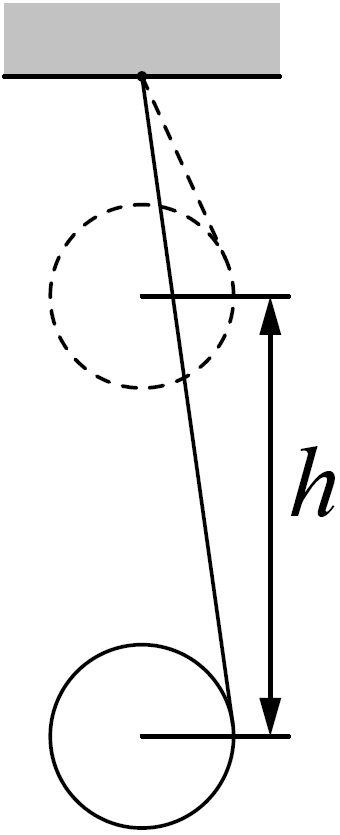
\includegraphics[height=5cm]{images/204_0.png}
    \caption{Versuchsaufbau Aufgabe 204}
\end{figure}
Die Kraft $F$, welche die Walze beschleunigt, ergibt sich aus der Seilkraft $F_S$ (nach oben) und der Gravitationskraft $F_G$ (nach unten).
\begin{align}
    F&=F_G-F_S					\nonumber\\
    m\cdot a &= m\cdot g - F_S	\nonumber\\
    F_S&=m\cdot(g-a)			\label{eq:204_force}
\end{align}
Die an der Walze anliegende Seilkraft erzeugt mit dem Radius $r$ der Walze ein Drehmoment $M$.
\begin{align}
    M=F_S\cdot r	\label{eq:204_torque0}
\end{align}
Für dieses gilt mit dem Trägheitsmoment $J$ und der Winkelbeschleunigung $\alpha$:
\begin{align}
    J&=\frac{m\cdot r^2}{2}			\nonumber\\
    \alpha&=\frac{a}{r}				\nonumber\\
    M&=J\cdot \alpha				\nonumber\\
    M&=\frac{m\cdot a\cdot r}{2}	\label{eq:204_torque1}
\end{align}
Setzt man nun \eqref{eq:204_force} in \eqref{eq:204_torque0} und die resultierende Gleichung mit \eqref{eq:204_torque1} gleich, erhält man:
\begin{align*}
    m\cdot(g-a)\cdot r&=\frac{m\cdot a\cdot r}{2}\\
    g-a&=\frac{a}{2}\\
    a&=\frac{2}{3}g\\
    &\boxed{a=6.54\frac{m}{s^2}}	\tag{a}\label{eq:204_a}
\end{align*}
Das Fallen der Walze ist eine gleichmäßig beschleunigte Bewegung. Dabei lässt sich folgende Aussage über das Verhältnis zwischen Start- und momentaner Geschwindigkeit treffen:
\begin{align*}
    v^2-v_0^2=2\cdot a\cdot s
\end{align*}
Da sich die Walze initial in Ruhelage befindet beträgt $v_0=0\frac{m}{s}$. Die zurückgelegte Strecke $s$ ist die Fallhöhe $h$.
\begin{align*}
    v^2&=2\cdot a\cdot h\\
    v&=\sqrt{2\cdot a\cdot h}\\
    v&=\sqrt{\frac{4\cdot g \cdot h}{3}}\\
    v&=\sqrt{\frac{4\cdot 9.81\frac{m}{s^2} \cdot 2m}{3}}\\
    &\boxed{v=5.11\frac{m}{s}}	\tag{b}	\label{eq:204_b}
\end{align*}
Da die Bewegung gleichmäßig beschleunigt ist, gilt dementsprechend:
\begin{align*}
    s&=\frac{a}{2}\cdot t^2+v_0\cdot t+s_0
\end{align*}
\newpage
Wie bereits erwähnt ist $s=h$ und die Anfangsgeschwindigkeit $v_0=0\frac{m}{s}$. Außerdem ist $s_0=0m$.
\begin{align*}
    h&=\frac{a}{2}\cdot t^2\\
    t^2&=\frac{2\cdot h}{a}\\
    t&=\sqrt{\frac{2\cdot h}{a}}\\
    t&=\sqrt{\frac{3\cdot h}{g}}\\
    t&=\sqrt{\frac{3\cdot 2m}{9.81\frac{m}{s^2}}}\\
    &\boxed{t=0.78s}	\tag{c}	\label{eq:204_c}
\end{align*}
Das Verhältnis von Zugkraft und Gewichtskraft ist beschrieben durch:
\begin{align*}
    \frac{F_S}{F_G}&=\frac{m\cdot(g-a)}{m\cdot g}\\
    \frac{F_S}{F_G}&=\frac{g-\frac{2}{3}g}{g}\\
    &\boxed{\frac{F_S}{F_G}=\frac{1}{3}}	\tag{d}	\label{eq:204_d}
\end{align*}